\chapter{Future works}

In this work we mainly focused our efforts towards author attribution in its most straightforward form, i.e. we are given examples of the writing of a number of candidate authors and are asked
to determine which of them authored a given anonymous text \cite{koppel2009computational}.
This approach to author attribution has been the only one studied until the last decade, as it is already quite complex.
The enormous steps forward both in terms of modern computing power and in terms of studies of new models of machine learning, have allowed to leave the concept of classical attribution and explore some of the tasks still unsolved, presented in the research question of chapter 2 of this work. In order to let the reader have a clear idea of what are these possible scenarios that we might encounter while studying modern author attribution model, we are going to discuss each one briefly:
\begin{enumerate}
	\item There is no candidate set at all. In this case, the challenge is to provide as much demographic or psychological information as possible about the author. This is the profiling problem.
	\item There are many thousands of candidates for each of whom	we might have a very limited writing sample. This is the needle-in-a-haystack problem.
	\item There is no closed candidate set but there is one suspect.
	In this case, the challenge is to determine if the suspect is or is not the author. This is the verification problem.
\end{enumerate}

\paragraph{The profiling problem} The profiling problem requires a collection of datasets for the supervised classification approach that features demographic and psychological properties of the author. This type of task is quite challenging because of these assumptions just listed, especially if we are talking about large data collections with tens or hundreds of authors.

\paragraph{The verification problem} The verification problem is the most applicable in reality especially in the forensic field. This type of author attribution task, however, is the one that represents more challenges at the time of writing this work. In fact, the most difficult challenge to overcome successfully this task is to find the right balance between positive examples (i.e. belonging to a given author) and negative examples (potentially all the texts of any other author present in the dataset but also outside of it).
This leads to have a strong unbalance towards the negative samples that puts in great difficulty the accuracy of the resulting model.

\paragraph{The needle-in-haystack problem} The needle-in-haystack problem in fact is not a scenario so different from those encountered so far. The main difference from the classical approach is for the greater closeness towards real datasets, such as having few examples per author for a large number of authors (just for the sake of mentioning the datasets collected by social media). These documents are fundamentally very short, we only have to look at Twitter's 140-character limitations, and for this very reason present a major challenge in this field that has yet to be resolved.

\paragraph{The open set authorship attribution} One of the closest problems to being solved in this field of authorship attribution is undoubtedly moving from a closed set group of authors to an open set group of authors. This revolution in approach allows us to have a group of authors in the supervised training phase and a classifier who must take into account that in the testing phase it may have to deal with labels (i.e. authors in this case) that it has never seen in the training phase and classify them as unknown. This approach is complex because it puts together similarities between the verification problem and the needle-in-haystack problem with the classic approach of author attribution in a closed set.
During the study of our work we have tried to validate our approach by dealing also with a type of open set of author attribution.
In fact, we removed 10\% of the authors from each dataset in the training phase and moved them to the testing phase.
To give the reader a better understanding we show a practical example: for the dataset RCV1-50 with 50 authors, for each of them we collected 100 documents.
In the closed set authorship attribution approach we would have had a 50/50 split, i.e. 50 documents of each author would have gone in the training phase and 50 documents of each author in the testing phase, thus leading to a balanced splitting between the classes.
In the open set authorship attribution approach, we selected 5 of the 50 authors whose 100\% of the documents (i.e., 100 documents) we placed in the testing phase by moving them out of the training phase. We thus obtained an unbalanced splitting of classes with a total of 50 documents for 45 authors in the training phase (a total of 2250 documents) and 50 documents for 45 authors, adding 100 documents for each of the 5 remaining authors in the testing phase, ending up with a total of 2750 documents in the testing phase.
For the open set authorship attribution approach we used a One Vs Rest classifier from the python library $
sklearn.multiclass.OneVsRestClassifier$ i.e. we built a classifier for each author, giving his 50 documents as positive examples and all other documents belonging to the other authors as negative examples.
We then inserted an additional label in the training phase, marking it as \enquote{unknown author} for the testing phase.
The results obtained with the datasets selected in this work are shown in \autoref{fig:results_open_set}. We excluded the dataset from The Guardian Corpus as the number of authors in the full dataset was too small to allow for reliable results without introducing learning bias.

\begin{figure}[ht]
	\centering
	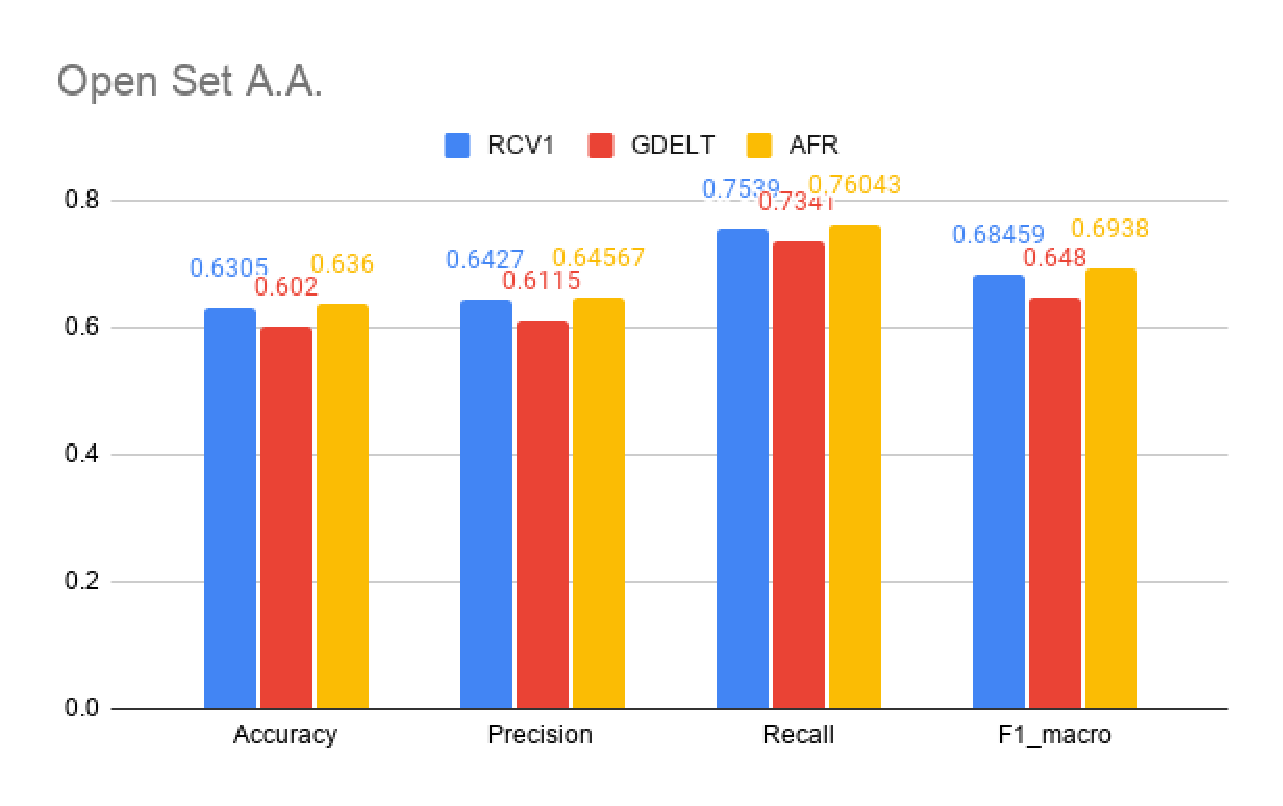
\includegraphics[width=0.8\textwidth, height=1.0\textheight, keepaspectratio]{open_set_aa}
	\caption[Results of our single topic dataset with open set authorship attribution]{Accuracy, precision, recall and f1-macro for Reuters Corpus, GDELT corpus and Amazon Food Reviews corpus for the open set authorship attribution task (10\% of unknown authors).}
	\label{fig:results_open_set}
\end{figure}

As we can see from the results obtained, there is a lot of room for improvement in terms of accuracy. In fact, we obtained results up to almost 25\% lower than the values obtained for the datasets considering the closed set authorship attribution problem.
These considerations made us mainly focus on the classical approach, but they give us the idea that many studies could come out on this particular type of authorship attribution subtask in the next years, as we have not yet found a valid approach that works for all types of datasets and for different authors set size.